In this section we will deal with the problem of placing side chains
on the protein and selecting side-chain conformations in a way that
minimizes the number of collisions.

As we mentioned in Section \ref{chap:protein_geometry}, statistical
analysis has shown that each type of amino acid side-chain has a small
set of common conformations \cite{dunbrack2002rotamer}. A side-chain
conformation is a configuration of its $\chi$ angles and is called a
\textit{rotamer}.

There has been developed several \textit{rotamer libraries}
\cite{dunbrack1997bayesian, lovell2000penultimate}, containing lists
of the common rotamers for each side-chain together with a probability
of each of those rotamer occuring in a protein. A comparison of some,
but not the most recent, rotamer libraries can be found in
\cite{dunbrack2002rotamer}. We have selected to use the rotamer
library made by Dunbrack et al. for the SCWRL side-chain
predictor\footnote{We use the latest release from 15th May 2002}.

\section{Our approach}
We have devised a simple algorithm for selecting side-chain rotamers,
with the goal of minimizing the number of collisions between
atoms. Our first step is to apply the rotamer from the rotamer library
with highest probability to each amino acid in the protein. After
this, we go through each amino acid, this time trying to eliminate
eventual collisions. We use a breadth-first search through a tree that
represents the eventual collisions occuring for the different rotamers
of the amino acids. On Figure \ref{fig:rotamer-search-tree} we have
illustrated how our algorithm progresses, when trying to remove
collisions with a single amino acid. Each vertex represents an amino
acid and each edge represents a collision between the node and its
child. The names on the edges represents rotamers of the node
above. As an example, when rotamer $3$ is applied to amino acid
\textit{a}, \textit{a} collides with both \textit{c} and \textit{d}.

The breadth-first search proceeds through each level, from the most
probable rotamer to the least probable (left-to right on the figure),
until a solution is found or a maximum depth is reached. For example,
we can resolve the collision in Figure~\ref{fig:rotamer-search-tree}
when rotamer $1$ is applied to \textit{a} and rotamer $3$ is applied
to \textit{b} the collision is solved. In the case where the amino
acid collides with more than one other amino acid, we stop as soon one
of the collisions is solved and postpone the solution of the remaining
collisions to we reach one of the collidees we haven't handled.

%% Hvornår kigger vi på rotameren som /a/ startede ud med at have?

\begin{figure}
	\centering
	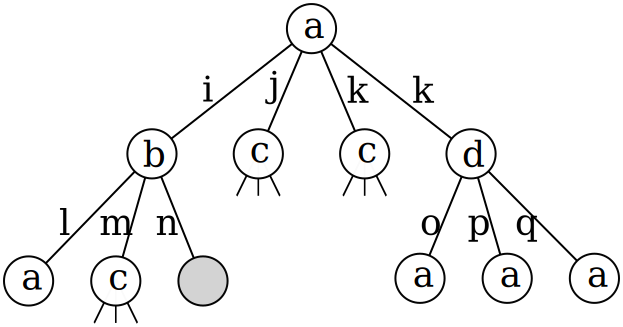
\includegraphics[width=.9\columnwidth]{figures/rotamersearch}
	\caption{The structure of our rotamer search space when eliminating
      collisions with the amino acid \textit{a}.}
    \label{fig:rotamer-search-tree}
\end{figure}

\section{Related Work}
The side-chain placement problem has been investigated by several
research groups, what we found most notably is the work done by
Dunbrack Labs on the SCWRL project \cite{canutescu2003graph,
  krivov2009improved}. The central algorithm in SCWRLs collision
resolving uses an \textit{interaction graph}, which much like our tree
has a vertex for each amino acid, but instead of the edges
representing that there currently is a collision, the graph has edges
between two amino acids if they \textit{could} collide by applying
certain rotamers on either or both of the amino acids. This graph can
be used to find clusters of interacting residues (two residues can
interact if there is a path between them). Large clusters cant be
solved efficiently, but they a cluster can be partitioned if there
exists what is called \textit{keystone vertices}
or\textit{articulation points} a which when removed breaks the graph
into two seperate subgraphs. For each rotamer of the keystone residue
the two subproblems can be solved. The rotamer of the keystone residue
which results in the lowest amount of free energy for the complete
cluster. Remark here that they use energies to evaluate the best
rotamer where as we have limited us from dealing with energy
functions and instead concentrate on the number of collisions.

In addition to this central algorithm, SCWRL has further advantages
over our algorithm. They use a lot of effort to delimit their search
space e.g. by removing rotamers with high self-energy from the set of
possible rotamers, where as we haven't focused at all on performance
in our implementation. SCWRL also tries to resolve whether any
collisions can be transformed into disulfide bridges, which are bonds
between two Cysteine amino acids (only pairs of Cysteine residues can form
disulfide bridges) from different places on the amino acid sequence
but spatially near each other.

%%% Local Variables: 
%%% mode: latex
%%% TeX-master: "rapport"
%%% End: 
